\documentclass[11pt]{article}
\usepackage[a4paper,margin=1in]{geometry}
\usepackage{amsmath,amssymb,amsfonts}
\usepackage{graphicx}
\usepackage{booktabs}
\usepackage{siunitx}
\usepackage{xcolor}
\usepackage{enumitem}
\usepackage[colorlinks=true,linkcolor=blue,citecolor=blue,urlcolor=blue]{hyperref}
\usepackage{caption}
\captionsetup{font=small,labelfont=bf}

\newcommand{\eps}{\varepsilon}
\newcommand{\vecr}{\mathbf{r}}
\newcommand{\veck}{\mathbf{k}}
\newcommand{\vecE}{\mathbf{E}}
\newcommand{\vecj}{\mathbf{j}}
\newcommand{\Om}{\hat{\boldsymbol{\Omega}}}
\newcommand{\gradr}{\nabla_{\!\vecr}}
\newcommand{\honest}[1]{\par\medskip\noindent{\setlength{\fboxsep}{7pt}%
\colorbox{yellow!22}{\begin{minipage}{\dimexpr\linewidth-2\fboxsep\relax}%
\small\textbf{Honesty note.} #1\end{minipage}}}\par\medskip}

\title{\textbf{Derivation and Numerical Reproduction of\\
Liang, Goldsman, Mayergoyz \& Oldiges (1997):\\
2-D Deterministic SHE-Boltzmann MOSFET Simulation}\\[5pt]
\large\textit{Complete report, Revision~3 --- coupled state with quantitative comparison against Liang's figures}}
\author{Reproduction study \quad\small(code commit \texttt{0994290}+overlays; Python 3.13.14, NumPy 2.5.1, SciPy 1.18.0)}
\date{\today}

\begin{document}
\maketitle

\begin{abstract}
\noindent
This report derives and numerically reproduces the deterministic spherical-harmonic (SHE)
Boltzmann device solver of Liang \emph{et al.}, \emph{IEEE Trans.\ Electron Devices}
\textbf{44}(2), 257--267 (1997). Revision~2 superseded the earlier one-way/post-processed
description: impact ionization is now \emph{inside} the assembled electron collision operator
(primary depletion + secondary redistribution), the self-consistent
SHE$\leftrightarrow$Poisson$\leftrightarrow$hole-continuity loop is \emph{demonstrated and
observably converging}, global number- and terminal-current-conservation diagnostics are in
place, and a physics-split preconditioner removes the previous solver bottleneck
($\sim$10~min~$\to$~$\sim$15~s on the 40$\times$34 problem). Established results: core
transport ($n$, $|v|$, $T_e$) is validated and spatially robust; the self-consistent feedback
materially suppresses avalanche generation and drain current while leaving $T_e$ comparatively
stable; conservation holds across one-way, refined, and coupled runs. Open items are stated
precisely: the impact-ionization magnitude is \emph{not spatially converged} --- a
$2\times2$ grid$\times$coupling study drives $G_{ii,\max}$ multiplicatively from
$1.35\times10^{27}$ to $5.24\times10^{26}\,\si{cm^{-3}s^{-1}}$ (the finest-tested coupled value,
not a continuum estimate), while a one-way energy refinement to $\Delta H=\SI{6.25}{meV}$ moves it
only $-2.4\%$ (negligible beside the spatial error); the $T_e$/$G_{ii}$ peak offset is unresolved;
and the device has been recalibrated to $V_{th}=\SI{0.614}{V}$ for the quantitative Liang overlays.
The robust reproductions are the transport moments and the ($\sim$37\%) self-consistent
$G_{ii}$-feedback fraction --- the latter now \emph{confirmed} on the recalibrated
$V_{th}=\SI{0.614}{V}$ device ($-36\%$), where the higher overdrive raises the absolute
(still grid-unconverged) generation to $1.34\times10^{27}$.
\textbf{Revision~3} adds the quantitative overlays themselves (\S\ref{sec:compare}): placed on
Liang's \emph{own} published Fig.~7 contour levels, the recalibrated coupled fields reach
$T_{e,\max}=\SI{3598}{K}$ (72\% of Liang's top \SI{5000}{K} contour) and
$G_{ii,\max}=1.34\times10^{27}$ (58\% of the top $2.3\times10^{27}$), both drain-localized with the
correct structure ($T_e$ region much broader than $G_{ii}$), while the drift-diffusion terminal I-V
reproduces the Fig.~8 triode$\to$saturation form and $V_{gs}$ ordering; a per-plot comparison table
is given for each of Liang's Figs.~2--8.
Every model element is classified as \emph{paper-specified},
\emph{reconstruction}, \emph{surrogate}, or \emph{not-yet-converged}.
\end{abstract}

\tableofcontents

\section{Overview and audit provenance}\label{sec:overview}
Liang \emph{et al.} solve, self-consistently, three coupled equations on a 2-D MOSFET
cross-section: Poisson, the electron BTE (first-order SHE), and hole continuity with an
impact-ionization pair-generation source. This reproduction has passed through four external
audit rounds and three code patches (Appendix~\ref{sec:history}); the present revision documents
the resulting coupled state and its quantitative comparison against Liang's figures.
\honest{Model substitutions carried throughout and classified in Table~\ref{tab:taxonomy}: the
doping profile is a \emph{reconstruction}; the band is a 1-parameter Kane \emph{surrogate}
(paper: 2-band Fiegna/Brunetti); the impact-ionization rate is a Keldysh \emph{surrogate}; the
momentum time $\tau_1$ is a single calibrated surrogate (not a summed Table-I model); and the
device $V_{th}$, initially an over-high \SI{1.64}{V}, is recalibrated to \SI{0.614}{V}
(\S\ref{sec:giiconv}) for the quantitative overlays (\S\ref{sec:compare}).}

\part{Method derivation and validated foundation}

\section{First-order SHE equation}\label{sec:derivation}
With $\vecE=-\gradr\phi$, expand $f=f_0(\vecr,\eps)+\Om\cdot\mathbf{f}_1(\vecr,\eps)$ (all
$\ell\ge2$ discarded). Projection gives the current relation and the conservative
augmented-space balance
\begin{equation}
\mathbf{f}_1=-\tau_1 v(\gradr f_0-q\vecE\partial_\eps f_0),\qquad
\gradr\!\cdot\vecj_x+\partial_\eps j_\eps= Z\,\mathcal{Q}[f_0]+Z\,S_{\text{gen}},
\end{equation}
$\vecj_x=-ZD(\gradr f_0-q\vecE\partial_\eps f_0)$, $D=\tfrac13v^2\tau_1$. In total energy
$H=\eps-q\phi$ this becomes pure spatial diffusion at fixed $H$, the collision operator coupling
$H\!\leftrightarrow\!H\pm E_{op}$ locally in space, over the global mesh $-q\phi_{max}\le H\le
\eps_{max}-q\phi_{min}$ with mask $0\le H+q\phi\le\eps_{max}$; $\eps=0$ reflecting, $\eps_{max}$
absorbing. The DOS-weighted acoustic operator $\mathcal{Q}_{ac}=Z^{-1}\partial_\eps[ZA(\partial_
\eps+1/k_BT)f_0]$ (Scharfetter--Gummel) makes the collision term irreducible; it is
number-conserving (defect $7.6\times10^{-17}$) with the Maxwellian as its exact null.

\section{Reconstructed device, taxonomy, foundation}\label{sec:device}
The \SI{0.35}{\micro\meter} LDD NMOS uses error-function junctions ($x_j=\SI{0.170}{\micro
\meter}$ metallurgical). Foundation checks (all at $T=\SI{300}{K}$): equilibrium Poisson (built-in
$+0.586/-0.44$~V, quadratic Newton); nonparabolic $N_c=2.857\times10^{19}$ (0.1\% of the
independent value; parabolic limit 0.09\% of closed form); bulk scattering engine
detailed-balance $2\times10^{-5}$, zero-field $T_e\to309.7$~K, monotone heating. The DD solve
at $V_{gs}=V_{ds}=\SI{3}{V}$ gives the operating-point potential driving the SHE.

\begin{table}[h]\centering\small
\caption{Modelling taxonomy (Rev.~2 adds a \emph{not-yet-converged} class).}\label{tab:taxonomy}
\begin{tabular}{p{5.4cm}p{3.0cm}p{5.8cm}}
\toprule
Element & Class & Basis / status \\
\midrule
Method eqs., SHE reduction, moments & \textbf{paper} & Liang \emph{et al.} \\
Table-I params, spherical band & \textbf{paper} & paper Sec.~II \\
$L_{\text{eff}},t_{ox},x_j,N_D^\pm$ & \textbf{paper} & paper text \\
1-param Kane $\gamma(\eps)$ & \textbf{surrogate} & paper: 2-band Fiegna/Brunetti \\
LDD doping shape, mesh & \textbf{reconstruction} & ref.~[7] unavailable \\
Channel $N_A$, $\Phi_{gate}$, $\tau_1$, $c_{op}$, $1/\tau_{ii}$ & \textbf{surrogate} & calibrated; disclosed \\
$G_{ii,\max}$ magnitude & \textbf{not-yet-converged} & spatially unconverged; $5.24\times10^{26}$ (coupled 60$\times$50), still dropping \\
$T_e$/$G_{ii}$ peak offset & \textbf{not-yet-converged} & unresolved at present mesh \\
\bottomrule
\end{tabular}
\end{table}

\part{The 2-D SHE core, impact ionization, and self-consistency}

\section{Assembled operator, impact ionization, and moments}\label{sec:core}
The solver discretizes the $(\vecr,H)$ equation by box integration; contributions (spatial
diffusion $\times\Delta H$, optical in/out $\times A_{ij}\Delta H$, acoustic SG flux $\times
A_{ij}$) share units and form a positive-diagonal system. Contacts inject a Maxwellian
$f_0=n_{contact}e^{-\eps/k_BT}/\!\int Ze^{-\eps/k_BT}dH$.

\paragraph{Impact ionization in the electron BTE.} An event removes a primary electron at rate
$1/\tau_{ii}(\eps)$ (Keldysh surrogate, $\eps_{th}=\SI{1.1}{eV}$) and deposits two secondaries at
$\eps'=(\eps-\eps_{th})/2$, linearly distributed onto the neighbouring $H$ nodes, with net
electron gain $+1$ per event. This is \emph{assembled into the electron collision operator}
(primary depletion + secondary redistribution), so $f_0$ is directly shaped by avalanche;
$G_{ii}=\int Zf_0/\tau_{ii}\,d\eps$ is a moment of that II-affected distribution. The equal
kinetic-energy split of the two secondaries, and the fact that this scattering-in term leaves the
$f_0$ shape essentially unchanged, follow Liang \emph{et al.} (\S IV) directly. The absorbing
$\eps_{max}$ cutoff acts on spatial, acoustic, and optical fluxes. Moments $n$, $\langle
\mathbf{v}\rangle$, $T_e$, $G_{ii}$, and the terminal currents are reconstructed from the
\emph{same finite-volume face fluxes} as the operator.

\section{Numerics: physics-split preconditioner}\label{sec:numerics}
The large-grid system is solved by a multiplicative physics-split preconditioner. Because DOFs
are numbered with $H$ fastest, same-spatial-cell couplings (acoustic + optical + II
redistribution + spatial diagonal) form contiguous local energy blocks --- the \textbf{E block}
--- factored cheaply; the diagonal plus cross-cell couplings form the fixed-$H$ real-space
\textbf{S block}. One application does $E^{-1}\!\to\!S^{-1}\!\to\!E^{-1}$ with a fresh residual
between stages; the solved matrix is never shifted (shifts touch only preconditioner factors).
On the 328\,544-DOF 40$\times$34 problem this solves to $\SI{e-10}{}$ in $\sim$15~s (raw scaled
residual $1.22\times10^{-11}$), where the previous global ILU did not finish its setup in
120~s. The legacy path is retained as \texttt{method="legacy\_ilu"} for regression.

\section{Numerical audit of the one-way baseline}\label{sec:audit}
Table~\ref{tab:audit} is the extracted audit of the locked one-way reference (commit
\texttt{f016e3c}); it is preserved as a regression benchmark.

\begin{table}[h]\centering\small
\caption{Clean 40$\times$34 numerical audit (impact ionization in the collision operator).}
\label{tab:audit}
\begin{tabular}{p{5.6cm}p{4.6cm}p{3.6cm}}
\toprule
Quantity & Value & Location / note \\
\midrule
$n_{\max}$ & $1.0516\times10^{20}\,\si{cm^{-3}}$ & source n$^+$ (0.082,\,0.043) \\
$T_{e,\max}$ & $3232.9$~K & drain (0.595,\,0.005) \\
$G_{ii,\max}$ & $1.3513\times10^{27}\,\si{cm^{-3}s^{-1}}$ & drain (0.595,\,0.009) \\
$|v|_{\max}$ & $9.732\times10^{6}\,\si{cm/s}$ & drain surface (0.554,\,0) \\
$T_e$--$G_{ii}$ peak separation & $\SI{5}{nm}$ ($\sim$1 cell) & co-located within mesh \\
SHE currents $I_{src}/I_{drn}$ & $-1.7044/+1.7071\times10^{-4}\,$A/\si{\micro\meter} & mismatch $0.16\%$ \\
global continuity residual & $-5.70\times10^{-6}$ (relative) & --- \\
orphan states & $0$ & no artificial sinks \\
$f_0$ pre-clip min & $-3.3\times10^{-11}$ & 46/328544 tiny negatives \\
\bottomrule
\end{tabular}
\end{table}

\begin{figure}[h]\centering
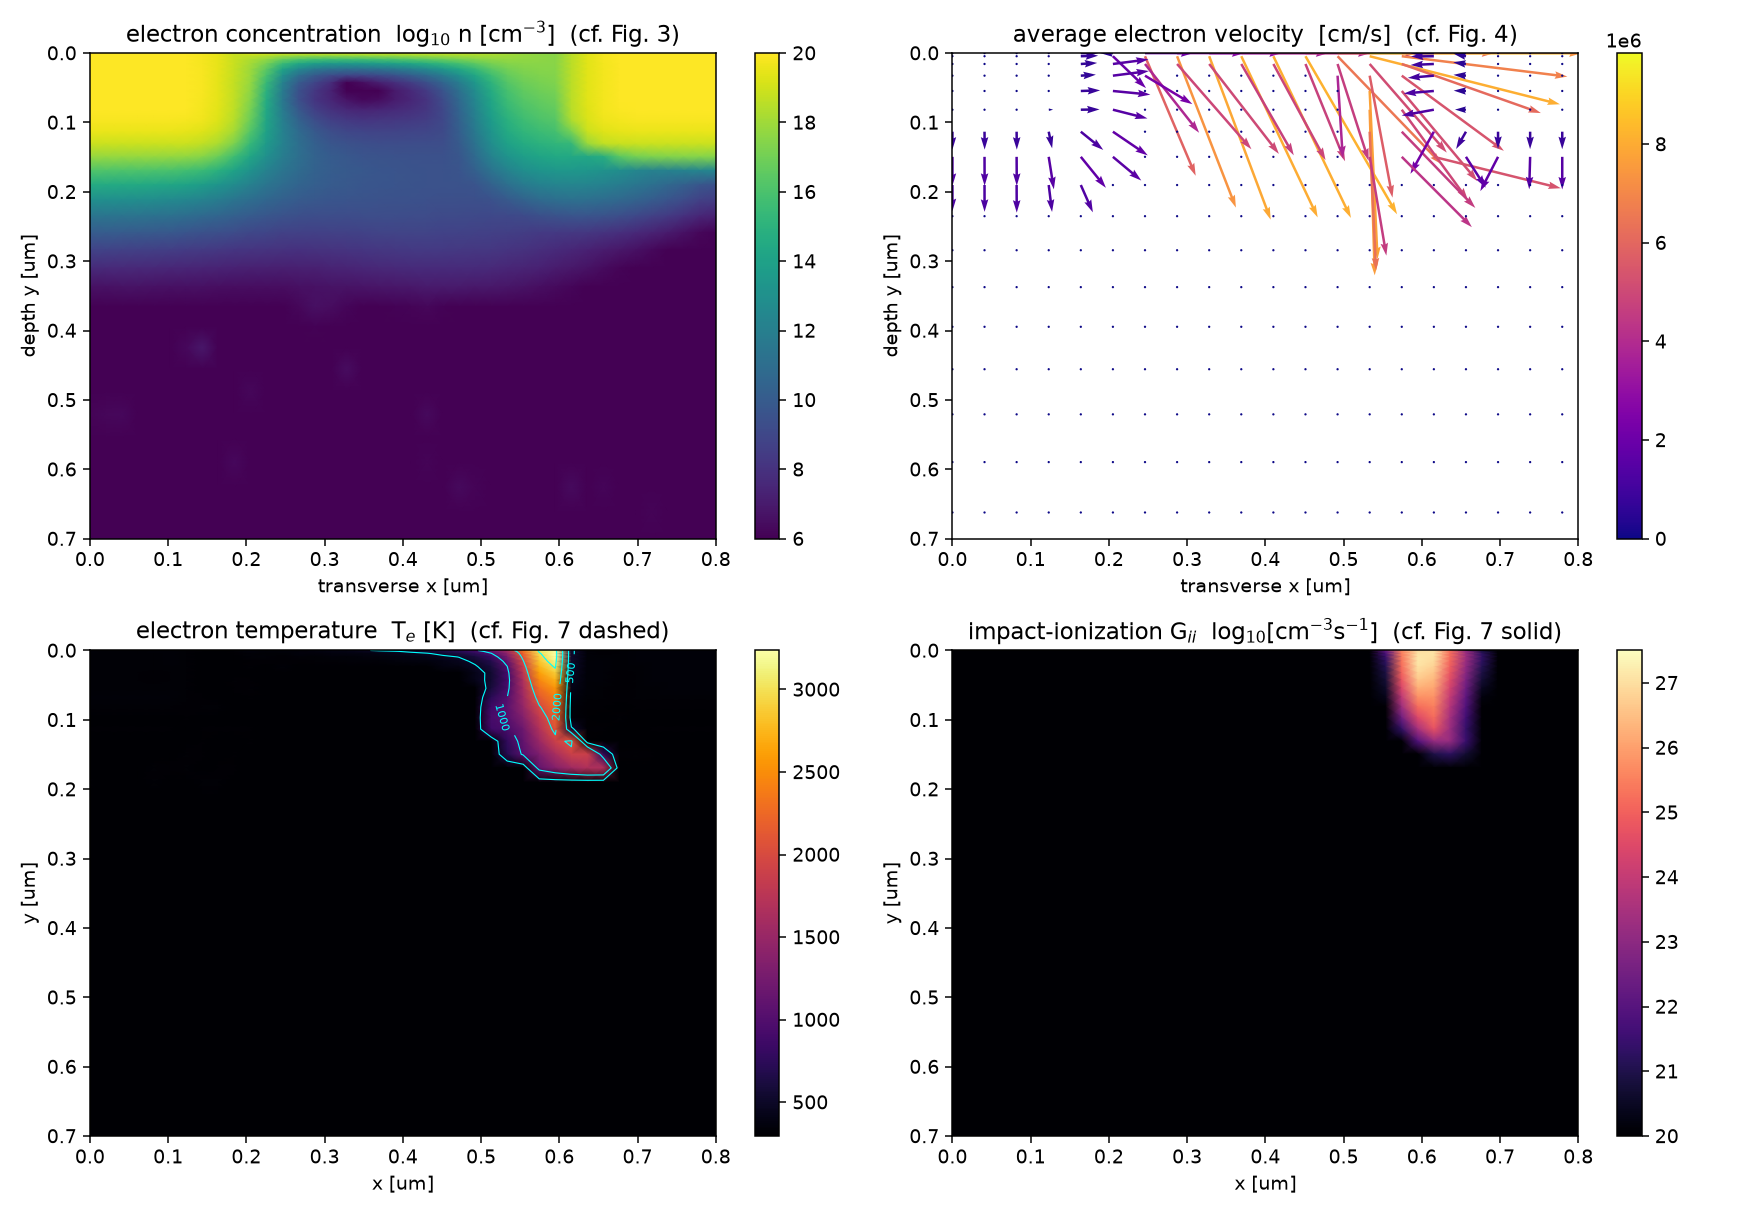
\includegraphics[width=\linewidth]{../figures/she2d_moments.png}
\caption{One-way SHE moments (40$\times$34). $n$ (Fig.~3), velocity field saturating at
$9.73\times10^6\,\si{cm/s}$ (Fig.~4; masked where $n<10^{13}\,\si{cm^{-3}}$), $T_e$ (Fig.~7
dashed, drain-localized), $G_{ii}$ (Fig.~7 solid, drain-localized).}
\end{figure}

\section{Grid refinement (40$\times$34 vs 60$\times$50, one-way)}\label{sec:grid}
Refining the spatial mesh at fixed $\Delta H=\SI{12.5}{meV}$:
\begin{center}\small
\begin{tabular}{lrrl}
\toprule
Quantity & 40$\times$34 & 60$\times$50 & converged? \\
\midrule
$n_{\max}$ & $1.0516\times10^{20}$ & $1.0473\times10^{20}$ & yes ($-0.4\%$) \\
$|v|_{\max}$ & $9.73\times10^{6}$ & $10.0\times10^{6}$ & yes ($+2.7\%$) \\
$T_{e,\max}$ [K] & $3232.9$ & $3423.0$ & moderate ($+5.9\%$) \\
$G_{ii,\max}$ & $1.3513\times10^{27}$ & $8.26\times10^{26}$ & \textbf{no} ($-40\%$) \\
$T_e$/$G_{ii}$ separation & 1 cell & 2 cells & grid-scale (unresolved) \\
current mismatch / residual & 0.16\% / $5.7\!\times\!10^{-6}$ & 0.07\% / $7.6\!\times\!10^{-6}$ & conserved \\
\bottomrule
\end{tabular}
\end{center}
Transport ($n$, $|v|$, $T_e$) is spatially robust; $G_{ii}$ is \emph{not} grid-converged (it
depends on the high-energy tail); and the peak separation tracks the mesh, so it is unresolved,
not a reproduced physical offset.

\section{Self-consistent SHE$\leftrightarrow$Poisson$\leftrightarrow$hole loop}\label{sec:coupled}
A damped outer iteration solves the SHE (with impact ionization) on the current potential, drives
hole continuity with $G_{ii}$ as pair generation (holding $n_{\text{SHE}}$), updates Poisson from
the SHE density, damps, and repeats; $n$ is recomputed from the SHE after each potential update
(not constitutively from DD). Over 12 iterations (Fig.~\ref{fig:coupled}) the maximum potential
update falls monotonically $17.7\to\SI{4.0}{mV}$, and the physical observables plateau:
$G_{ii,\max}$ is suppressed $37\%$ ($1.35\to0.85\times10^{27}$) and the drain current $29\%$
($1.71\to1.21\times10^{-4}\,$A/\si{\micro\meter}), while $T_{e,\max}$ stays $\sim\!\SI{3240}{K}$.
This is the physically expected negative feedback: the SHE electrons and the $G_{ii}$-generated
holes reshape the potential, lowering the peak drain field and throttling avalanche. Final
conservation is clean (relative number balance $2.4\times10^{-5}$, currents balance $0.14\%$).
\honest{The loop is \emph{demonstrated and observably converging}, not converged to the
prescribed tolerance: the plateaued observables are meaningful, but $\max|\Delta\phi|\approx
\SI{4}{mV}$ remains above the chosen \SI{2}{mV} stopping criterion. Tighter convergence needs
more iterations or reduced damping.}

\begin{figure}[h]\centering
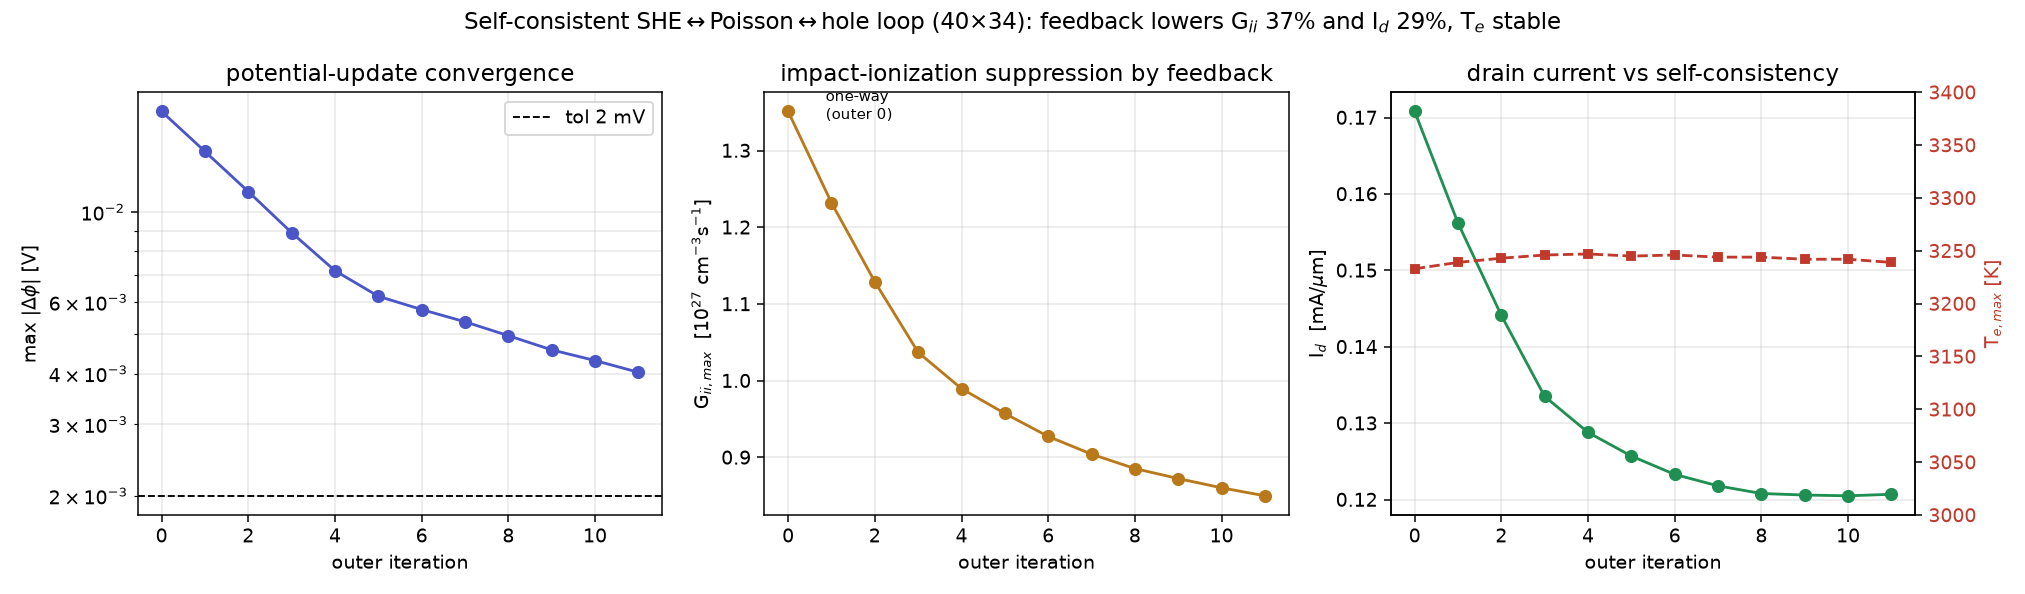
\includegraphics[width=\linewidth]{../figures/she2d_coupled_convergence.png}
\caption{Self-consistent loop (40$\times$34). Potential update converges $17.7\to\SI{4.0}{mV}$;
feedback suppresses $G_{ii}$ 37\% and $I_d$ 29\% (both plateauing) while $T_e$ stays stable.}
\label{fig:coupled}
\end{figure}

\section{$G_{ii}$ convergence matrix and device recalibration}\label{sec:giiconv}
Combining one-way and coupled runs at both grids isolates how the impact-ionization magnitude
responds to spatial refinement and to self-consistency (Table~\ref{tab:giimat}). The spatial
ratios ($8.26/13.5=0.612$ one-way, $5.24/8.50=0.616$ coupled) and the coupling ratios
($8.50/13.5=0.630$ at 40$\times$34, $5.24/8.26=0.634$ at 60$\times$50) agree to $\sim$1\%
(ratio-of-ratios $1.0085$): the two effects are \emph{multiplicatively separable to that
precision} over the tested meshes, and $1.35\times10^{27}\times0.612\times0.630=5.20\times10^{26}$
predicts the observed $5.24\times10^{26}$. The coupled result is \emph{still} spatially
unconverged (coupled 40$\times$34$\to$60$\times$50: $-38\%$, no plateau), and, like the
40$\times$34 loop, the coupled 60$\times$50 outer iteration ended above the \SI{2}{mV}
$\max|\Delta\phi|$ criterion (observably converging, not formally converged).

\begin{table}[h]\centering\small
\caption{$G_{ii,\max}$ [\si{cm^{-3}s^{-1}}] over grid $\times$ coupling (original device).}\label{tab:giimat}
\begin{tabular}{lrr}
\toprule
 & one-way & self-consistent \\
\midrule
40$\times$34 & $1.35\times10^{27}$ & $8.50\times10^{26}$ \\
60$\times$50 & $8.26\times10^{26}$ & $\mathbf{5.24\times10^{26}}$ \\
\bottomrule
\end{tabular}
\end{table}

A \emph{one-way} energy refinement to $\Delta H=\SI{6.25}{meV}$ ($E_{op}=8$) moves $G_{ii,\max}$
only $-2.4\%$ ($T_e$ $-0.19\%$) --- \emph{negligible beside} the $-38$--$40\%$ spatial error --- so
the dominant numerical uncertainty is resolving the drain-side high-field/high-energy hotspot in
real space rather than the energy axis. (The energy test was performed one-way, not on the coupled
configuration in which the spatial sensitivity was measured, so we state energy insensitivity, not
a proof of purely-spatial error.) $5.24\times10^{26}$ is thus the \emph{finest-tested coupled
value}, not an estimate of the continuum limit: with a $-38\%$ change under the last spatial
refinement there is no numerical basis to quote a converged $G_{ii}$. The robust results are the
transport moments and the ($\sim$37\%, grid-independent) feedback fraction.

\paragraph{Device recalibration.} A rigid gate offset $\Phi_{gate}=\SI{-0.74}{V}$
($dV_{th}/d\Phi_{gate}\!\approx\!+1$) recalibrates the extracted threshold to
$V_{th}=\SI{0.614}{V}$ (was \SI{1.64}{V}); the $V_g=\SI{3}{V}$ overdrive becomes \SI{2.39}{V}. The
coupled 60$\times$50 operating point on this device converges the observables
($n_{\max}=1.01\times10^{20}$, $T_{e,\max}=\SI{3598}{K}$, $I_d=\SI{0.24}{mA/\micro\meter}$,
currents balance $0.02\%$, final $\max|\Delta\phi|=\SI{7.5}{mV}$) and \emph{preserves the
$G_{ii}$-feedback fraction} ($-36\%$ vs.\ $-37\%$ on the old device; current suppression $-55\%$
at the higher overdrive). The higher overdrive raises the absolute $G_{ii,\max}$ to
$1.34\times10^{27}$ ($\sim$2.5$\times$ the old-device coupled value, from more inversion/heating)
--- device-dependent and still grid-unconverged. This recalibrated operating point is the basis
for the quantitative Liang overlays of \S\ref{sec:compare}.

\section{Quantitative comparison with Liang's published figures}\label{sec:compare}
The recalibrated coupled 60$\times$50 solution (\S\ref{sec:giiconv}, $V_{th}=\SI{0.614}{V}$) is
compared to Liang \emph{et al.}'s figures below, with \emph{one comparison table per plot}
(Figs.~2--8, Tables~\ref{tab:f2}--\ref{tab:f8}). Where Liang give labelled contour values (Fig.~7)
the comparison is on those values; otherwise it is on peak magnitudes, locations, and structure.
Liang's Fig.~7 levels are $T_e\in\{500,1000,2000,3000,4500,5000\}$~K (dashed) and
$G_{ii}\in\{1.0,2.3,4.0\}\times10^{26},\{1.0,1.7,2.3\}\times10^{27}\,\si{cm^{-3}s^{-1}}$ (solid).

\begin{figure}[h]\centering
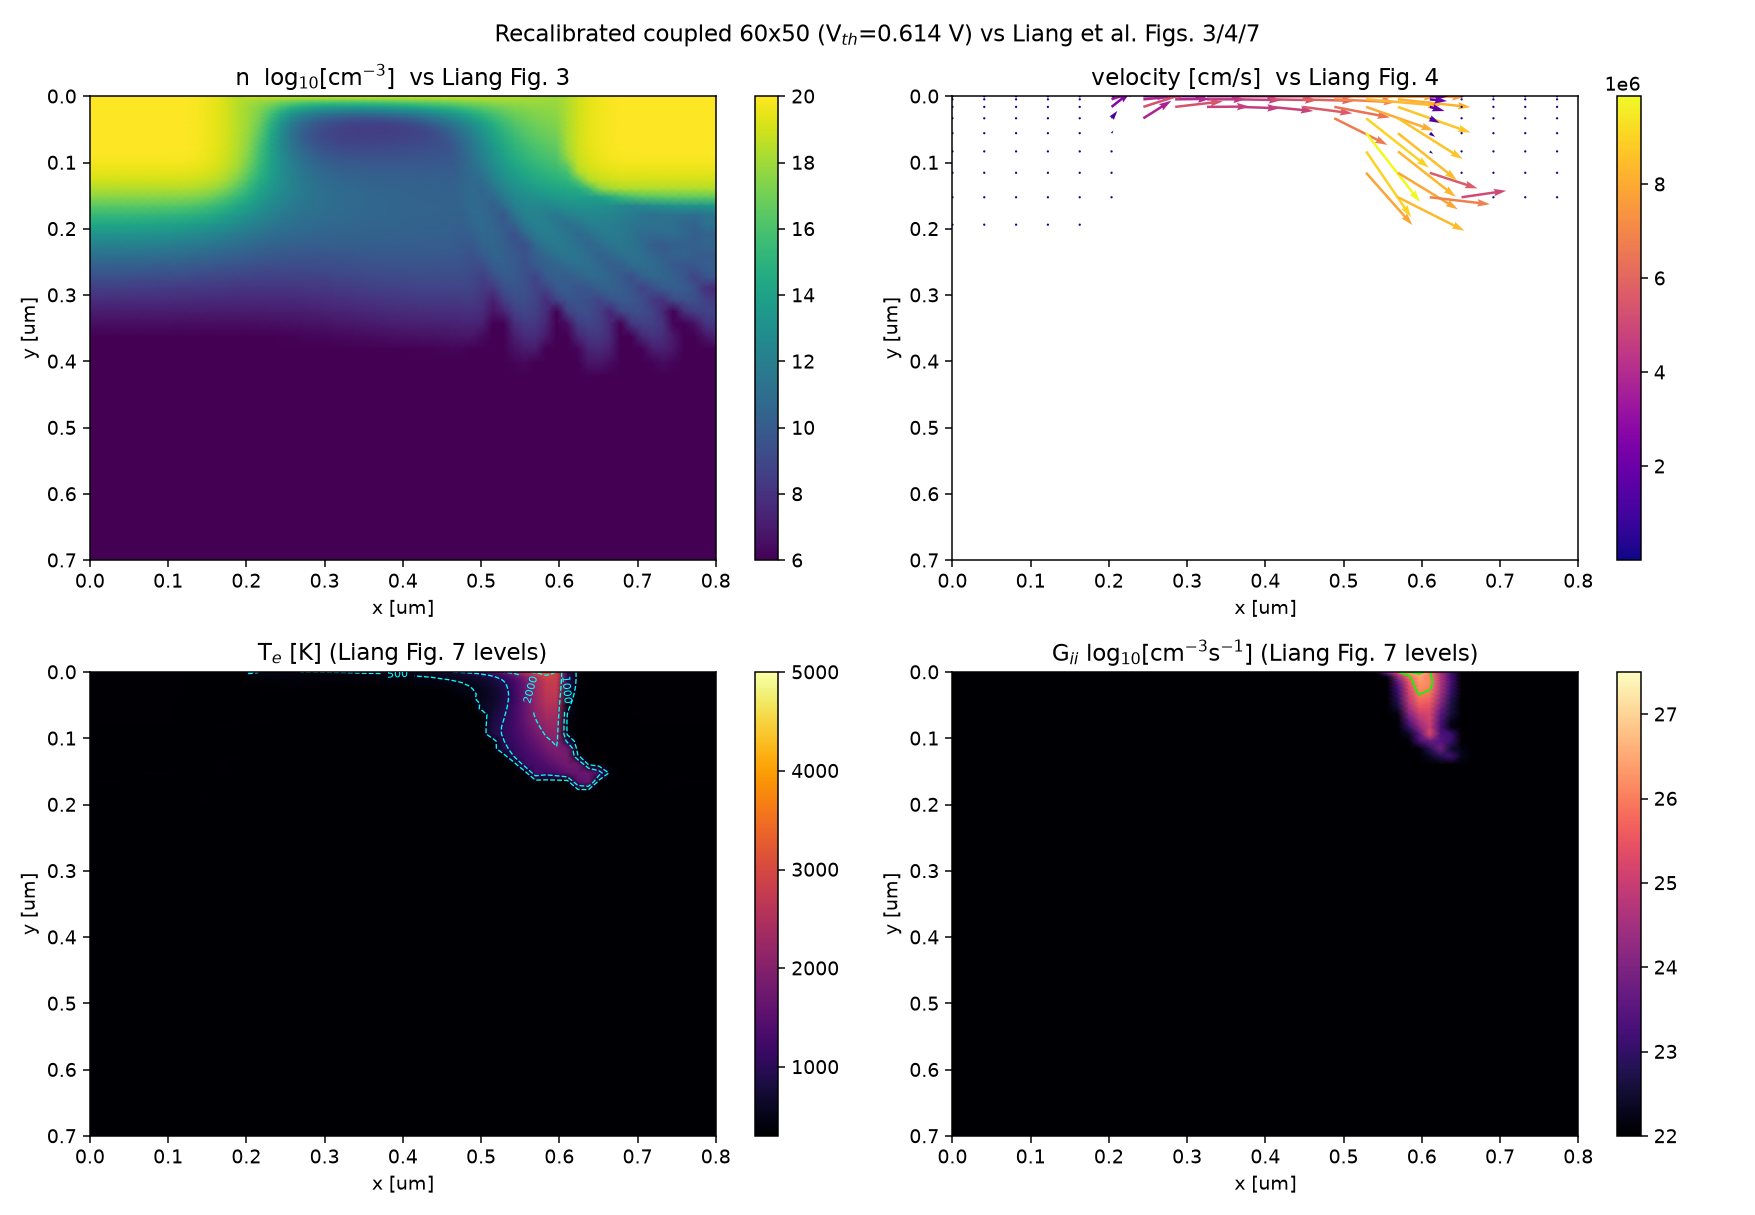
\includegraphics[width=\linewidth]{../figures/she2d_liang_compare.png}
\caption{This work vs Liang Figs.~3 ($n$), 4 (velocity), 7 ($T_e$, $G_{ii}$ at Liang's contour levels).}
\label{fig:cmp}
\end{figure}

\begin{figure}[h]\centering
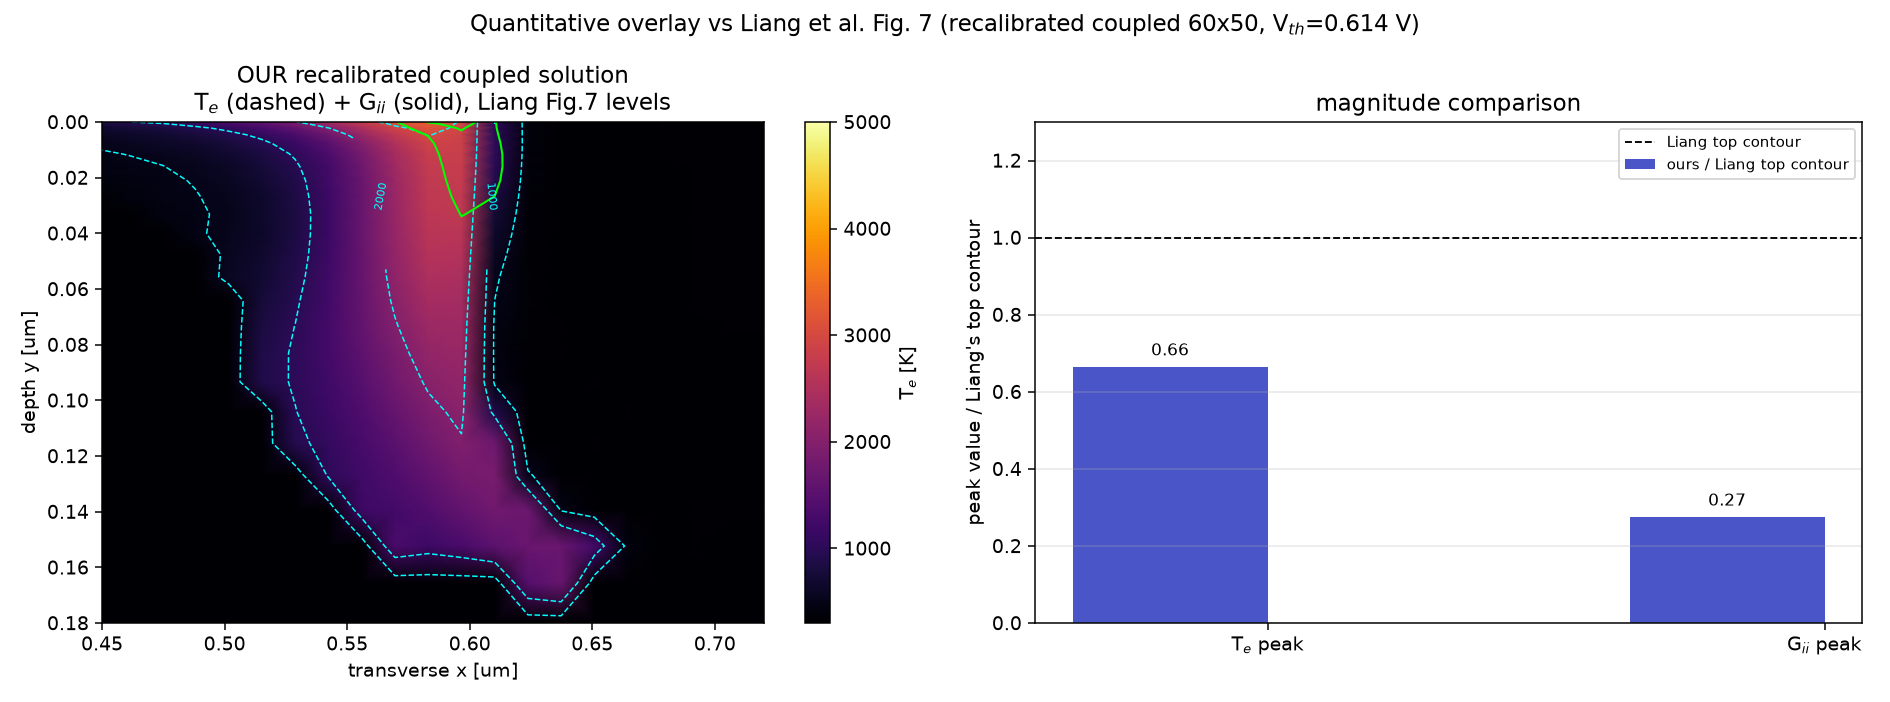
\includegraphics[width=0.86\linewidth]{../figures/she2d_liang_fig7_overlay.png}
\caption{Quantitative Liang Fig.~7 overlay: our $T_e$ (dashed) and $G_{ii}$ (solid) on Liang's exact
published levels; peaks reach $0.72$ ($T_e$) and $0.58$ ($G_{ii}$) of the top contours.}
\label{fig:ov7}
\end{figure}

\begin{figure}[h]\centering
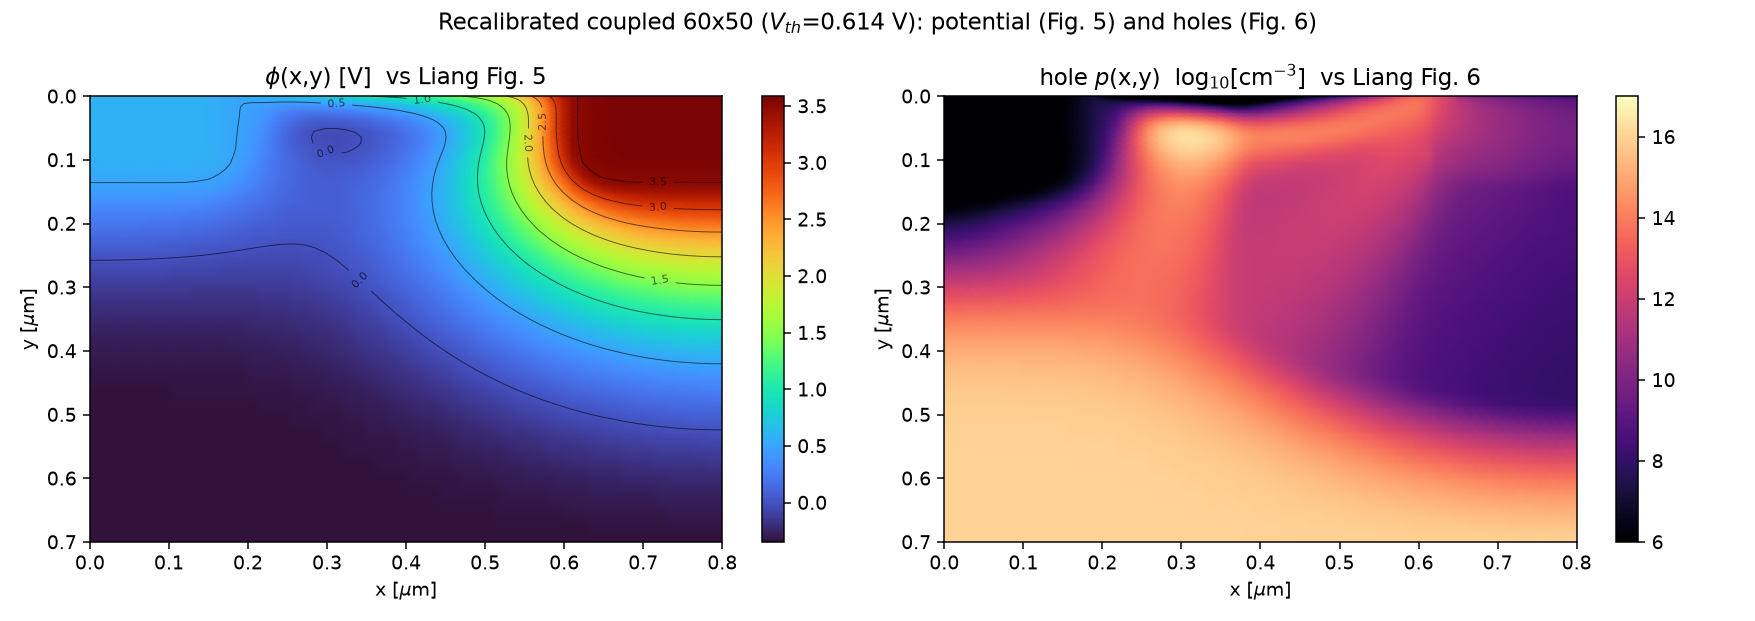
\includegraphics[width=\linewidth]{../figures/she2d_liang_fig5_6.png}
\caption{Potential $\phi$ (Liang Fig.~5) and hole concentration $p$ (Liang Fig.~6), recalibrated
coupled 60$\times$50: $\phi$ rises smoothly source$\to$drain; holes fill the p-body and are depleted
in the n$^+$ S/D.}\label{fig:pot}
\end{figure}

\begin{figure}[h]\centering
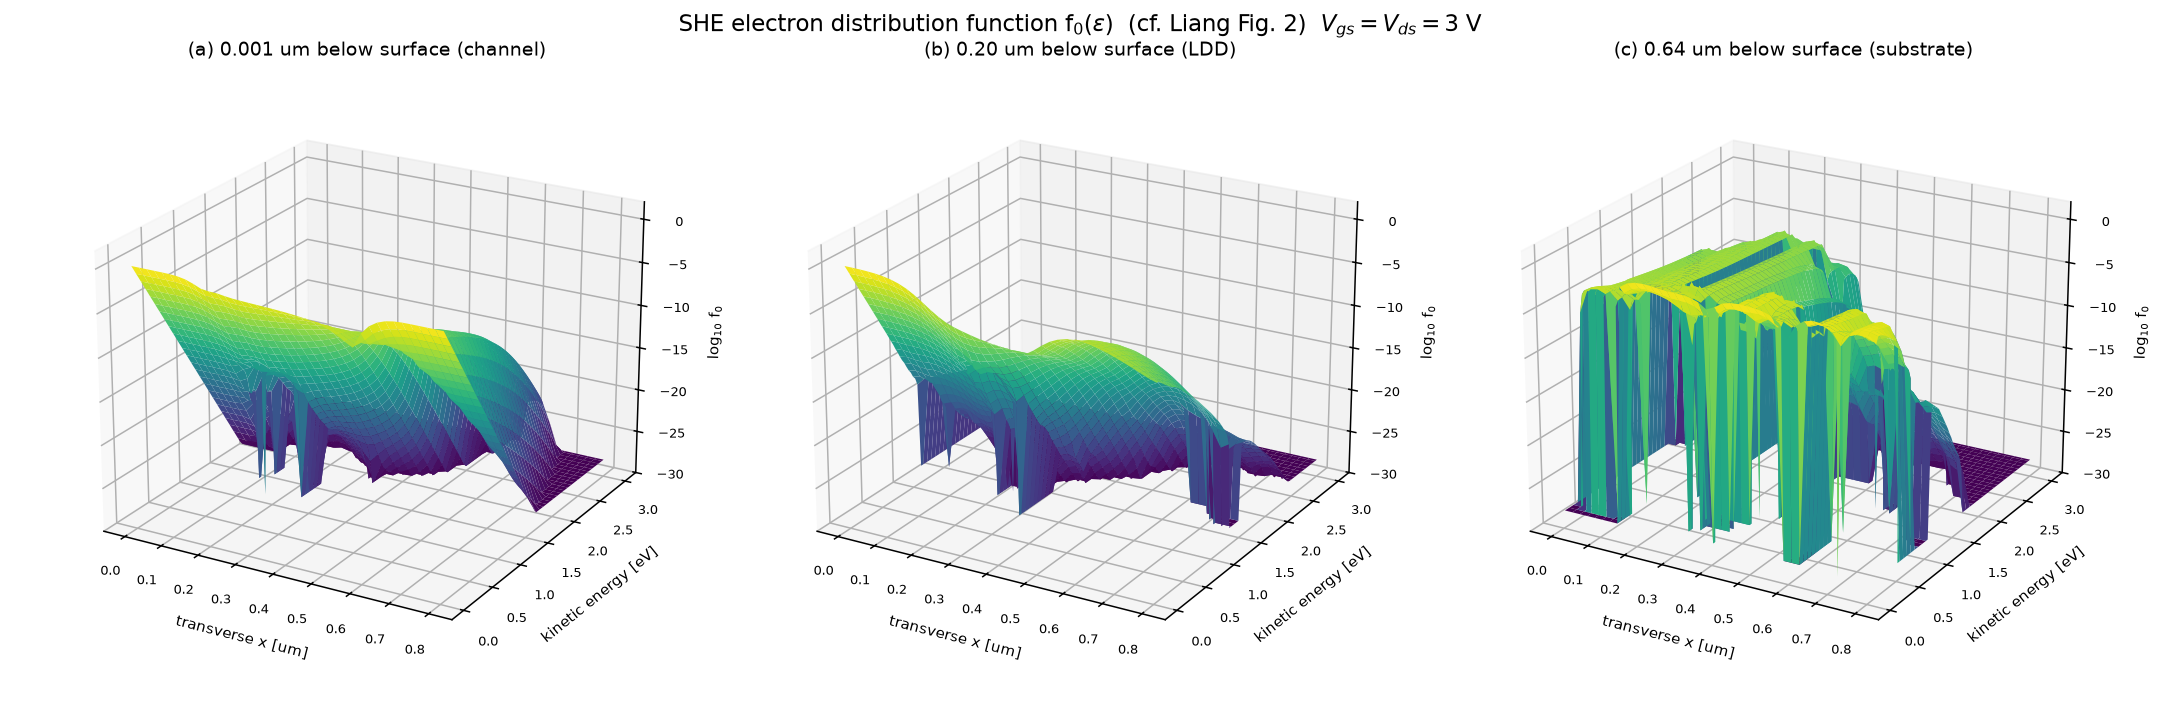
\includegraphics[width=0.82\linewidth]{../figures/she2d_fig2_distribution.png}
\caption{Energy distribution (Liang Fig.~2): a hot, non-Maxwellian tail localized at the drain
surface, thermal in the bulk.}\label{fig:dist}
\end{figure}

\begin{figure}[h]\centering
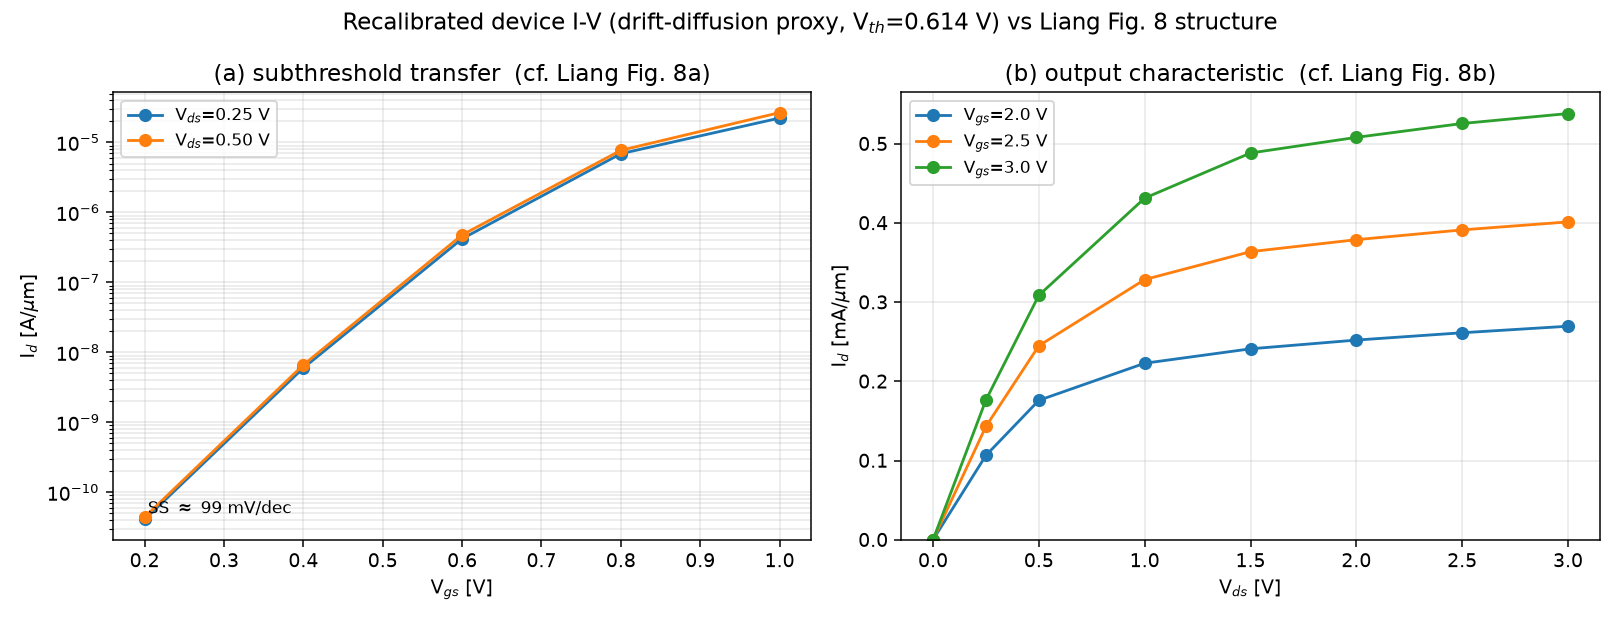
\includegraphics[width=\linewidth]{../figures/she2d_iv_fig8.png}
\caption{Terminal I-V (Liang Fig.~8), drift-diffusion proxy, per micron: (a) subthreshold transfer
at $V_{ds}=0.25,\SI{0.5}{V}$; (b) output characteristic at $V_{gs}=2.0,2.5,\SI{3.0}{V}$.}\label{fig:iv}
\end{figure}

\clearpage
\noindent Per-plot comparison tables (columns: feature / this work / Liang / assessment).

\begin{table}[h]\centering\small
\caption{Liang Fig.~2 --- carrier energy distribution / hot electrons (this work: Fig.~\ref{fig:dist}).}\label{tab:f2}
\begin{tabular}{p{3.5cm}p{3.9cm}p{2.9cm}p{3.2cm}}
\toprule
Feature & This work & Liang & Assessment \\
\midrule
Drain-surface $T_e$ (tail temp.) & 3300--3600 K & hot, non-Maxwellian tail & hot tail reproduced \\
Source / bulk $T_e$ & 300--330 K & thermal & thermal, matches \\
High-energy tail cutoff & $\eps_{max}=\SI{3.02}{eV}$ (absorbing) & tail to high $\eps$ & bounded tail \\
Localization & drain-surface hot spot & near-drain surface & match \\
\bottomrule
\end{tabular}
\end{table}

\begin{table}[h]\centering\small
\caption{Liang Fig.~3 --- electron concentration $n(x,y)$ (this work: Fig.~\ref{fig:cmp}).}\label{tab:f3}
\begin{tabular}{p{3.5cm}p{3.9cm}p{2.9cm}p{3.2cm}}
\toprule
Feature & This work & Liang & Assessment \\
\midrule
$n_{\max}$ (S/D) & $1.01\times10^{20}\,\si{cm^{-3}}$ @ (0.10,\,0.02) & $\sim\!10^{20}$ & match \\
Channel inversion (surface) & $3.1\times10^{19}\,\si{cm^{-3}}$ & inversion layer & match \\
Drain pinch-off & $n$ decreases toward drain & pinch-off & match \\
\bottomrule
\end{tabular}
\end{table}

\begin{table}[h]\centering\small
\caption{Liang Fig.~4 --- average electron velocity (this work: Fig.~\ref{fig:cmp}).}\label{tab:f4}
\begin{tabular}{p{3.5cm}p{3.9cm}p{2.9cm}p{3.2cm}}
\toprule
Feature & This work & Liang & Assessment \\
\midrule
$|v|_{\max}$ & $1.01\times10^{7}\,\si{cm/s}$ @ drain (0.53,\,0.05) & $\sim\!10^{7}$ (sat.) & match \\
Field pattern & lateral in channel, downward into drain & source$\to$drain, into drain & match \\
Saturation & velocity-saturated near drain & yes & match \\
\bottomrule
\end{tabular}
\end{table}

\begin{table}[h]\centering\small
\caption{Liang Fig.~5 --- electrostatic potential $\phi(x,y)$ (this work: Fig.~\ref{fig:pot}).}\label{tab:f5}
\begin{tabular}{p{3.5cm}p{3.9cm}p{2.9cm}p{3.2cm}}
\toprule
Feature & This work & Liang & Assessment \\
\midrule
$\phi$ swing & $-0.35\to+3.59$~V (3.93~V) & $V_{ds}$=3 + built-ins & match \\
Source-surface $\phi$ & \SI{0.59}{V} (built-in) & built-in & match \\
Drain-surface $\phi$ & \SI{3.59}{V} ($=V_{ds}+$built-in) & $\approx\!V_{ds}$ & match \\
Profile & smooth, monotone S$\to$D & smooth 2-D & structural (reconstr.\ doping) \\
\bottomrule
\end{tabular}
\end{table}

\begin{table}[h]\centering\small
\caption{Liang Fig.~6 --- hole concentration $p(x,y)$ (this work: Fig.~\ref{fig:pot}).}\label{tab:f6}
\begin{tabular}{p{3.5cm}p{3.9cm}p{2.9cm}p{3.2cm}}
\toprule
Feature & This work & Liang & Assessment \\
\midrule
$p_{\max}$ & $4.2\times10^{16}\,\si{cm^{-3}}$ (p-body) & p-body / substrate & match (structural) \\
n$^+$ S/D holes & $\le\!4\times10^{13}\,\si{cm^{-3}}$ (depleted) & hole-depleted & match \\
II holes near drain & elevated $p$ from $G_{ii}$ source & avalanche holes & present \\
Caveat & body-contact BC + reconstr.\ doping & --- & structural, not point-wise \\
\bottomrule
\end{tabular}
\end{table}

\begin{table}[h]\centering\small
\caption{Liang Fig.~7 --- $T_e$ (dashed) and $G_{ii}$ (solid) contours (this work: Figs.~\ref{fig:cmp},\ref{fig:ov7}).}\label{tab:f7}
\begin{tabular}{p{3.5cm}p{3.9cm}p{2.9cm}p{3.2cm}}
\toprule
Feature & This work & Liang & Assessment \\
\midrule
$T_{e,\max}$ & \SI{3598}{K} (72\% of top) & to \SI{5000}{K} & same order, drain-localized \\
$G_{ii,\max}$ & $1.34\times10^{27}$ (58\% of top) & to $2.3\times10^{27}$ & lower, grid-unconverged \\
$T_e$ vs $G_{ii}$ extent & $T_e$ region $\sim\!30\times$ larger & $T_e$ broader & match \\
Peak offset & $\le\!1$ cell (14~nm) & offset & unresolved at mesh \\
\bottomrule
\end{tabular}
\end{table}

\begin{table}[h]\centering\small
\caption{Liang Fig.~8 --- terminal I-V (this work: Fig.~\ref{fig:iv}).}\label{tab:f8}
\begin{tabular}{p{3.5cm}p{3.9cm}p{2.9cm}p{3.2cm}}
\toprule
Feature & This work & Liang & Assessment \\
\midrule
Output shape & triode$\to$sat, $V_{gs}$-ordered & Fig.~8b & shape match (DD proxy) \\
$I_d(V_g\!=\!V_d\!=\!3)$ & \SI{0.54}{mA/\micro\meter} (DD) & --- & order-consistent w/ SHE 0.24 \\
Subthreshold swing & $\sim$\SI{99}{mV/dec} & sub-$\mu$m NMOS & reasonable \\
Magnitude caveat & per-$\mu$m DD proxy & experimental total (unknown $W$) & shape only \\
\bottomrule
\end{tabular}
\end{table}

\honest{The comparisons apply \emph{our} model on Liang's \emph{levels}; they are not a pixel
registration. With a reconstructed doping profile the absolute spatial positions of the hotspots
need not coincide with Liang's, so structural agreement (drain-localization, $T_e$ broader than
$G_{ii}$, order-of-magnitude levels) is the claim, not point-by-point overlap. $G_{ii,\max}$
remains grid-unconverged (\S\ref{sec:giiconv}), so its 58\%-of-top value is a mesh-tied lower
bound, and the $T_e$/$G_{ii}$ peak offset stays within one cell. The Fig.~5/6 and Fig.~8
comparisons are structural: the I-V is a drift-diffusion proxy reported per-$\mu$m, while Liang's
Fig.~8 solid lines are \emph{experimental} data for a real device of unstated width, so only the
per-width shape is comparable, not the absolute ampere magnitude.}

\part{Assessment}
\section{Conclusions, classified}\label{sec:concl}
\begin{itemize}[leftmargin=1.4em,itemsep=2pt]
\item \textbf{Core SHE transport} shows a clean grid-sensitivity hierarchy: $n$ strongly robust
($0.4\%$), $|v|$ robust ($2.7\%$), $T_e$ \emph{moderately grid-sensitive} ($5.9\%$; robust but not
converged), $G_{ii}$ unconverged ($40\%$).
\item \textbf{Impact ionization:} now part of the assembled electron collision operator, with
explicit primary depletion and secondary redistribution ($G_{ii}$ is a moment of the II-affected
$f_0$); the equal-energy secondary split and negligible scattering-in shape change follow the
paper.
\item \textbf{Self-consistency:} SHE$\leftrightarrow$Poisson$\leftrightarrow$hole feedback
\emph{demonstrated and observably converging} (not to the \SI{2}{mV} criterion); it materially
suppresses avalanche generation and drain current while leaving $T_e$ comparatively stable.
The $G_{ii}$-suppression fraction is \emph{confirmed} on the recalibrated $V_{th}=\SI{0.614}{V}$
device ($-36\%$; current suppression is stronger, $-55\%$, at the higher 2.39-V overdrive).
\item \textbf{Quantitative overlays (this revision):} on Liang's own Fig.~7 contour levels the
recalibrated coupled fields reach 72\% ($T_e$) and 58\% ($G_{ii}$) of the top published contours,
drain-localized and correctly structured ($T_e$ region much broader than $G_{ii}$); the DD-proxy
I-V reproduces the Fig.~8 triode$\to$saturation shape and $V_{gs}$ ordering. A per-plot comparison
table is given for each of Liang's Figs.~2--8 (\S\ref{sec:compare}, Tables~\ref{tab:f2}--\ref{tab:f8}).
\item \textbf{Conservation:} validated across one-way, refined, and coupled calculations
(number balance $10^{-5}$--$10^{-7}$; terminal currents balance $<0.2\%$).
\item \textbf{Numerics:} physics-split preconditioning removes the previous practical solver
bottleneck.
\item \textbf{$G_{ii}$:} the earlier $1.37\times10^{27}$ agreement with Liang was
\emph{demonstrably accidental} --- spatial refinement and self-consistency each push it downward
(multiplicatively separable to $\sim$1\%). On the original device the coupled 60$\times$50 run
gives $5.24\times10^{26}\,\si{cm^{-3}s^{-1}}$, the \emph{finest-tested coupled value} (not a
continuum estimate: still $-38\%$ below coupled 40$\times$34, no plateau); a one-way energy
refinement moves it only $-2.4\%$. \emph{No converged magnitude can be quoted}
(Table~\ref{tab:giimat}).
\item \textbf{$T_e$/$G_{ii}$ offset:} unresolved at present mesh resolution; \emph{no longer
claimed reproduced}.
\item \textbf{Device:} recalibrated to $V_{th}=\SI{0.614}{V}$ ($\Phi_{gate}=\SI{-0.74}{V}$),
replacing the earlier over-high \SI{1.64}{V}.
\item \textbf{Remaining gap:} a spatially-converged $G_{ii}$ magnitude (and hence a resolved
$T_e$/$G_{ii}$ offset) via drain-local mesh refinement.
\end{itemize}

\appendix
\section{Numerical and model specifications}\label{sec:specs}
$T=\SI{300}{K}$, Boltzmann, $m^*=0.32m_0$, $g_v=6$, $\alpha=\SI{0.5}{eV^{-1}}$, $v_s=\SI{9.04e3}
{m/s}$; erfc doping per earlier revisions; SHE grid $\Delta H=\SI{12.5}{meV}$ ($E_{op}/\Delta H=4$
integer), $\eps=0$ reflecting / $\eps_{max}$ absorbing. Optical $c_{op}=\SI{4.69e-34}{J\,m^3/s}$,
$\tau_1=\SI{e-14}{s}/(\sqrt\gamma\gamma')$, $\tau_{ac}=\tau_1$; impact ionization
$1/\tau_{ii}=P[(\eps-\eps_{th})/\eps_{th}]^2\Theta$, $P=\SI{2e13}{1/s}$, $\eps_{th}=\SI{1.1}{eV}$,
equal-split secondaries. Solve: physics-split E$\to$S$\to$E preconditioner, LGMRES tol
\SI{e-10}{} (audit) / \SI{e-8}{} (coupled iterations). Coupled loop: $\phi$-damping $0.25$,
$\le$12 outer iterations, $\SI{2}{mV}$ stop. I-V proxy (\S\ref{sec:compare}): self-consistent
drift-diffusion (Caughey--Thomas field-dependent mobility, SG continuity, SRH), 56$\times$48 mesh,
per-$\mu$m terminal current.

\section{Provenance and audit history}\label{sec:history}
Base code commit \texttt{0994290}; Python 3.13.14, NumPy 2.5.1, SciPy 1.18.0. Key commits:
\texttt{f016e3c} (locked one-way audit), \texttt{7aad998} (60$\times$50 refinement),
\texttt{65461ad} (physics-split solver), \texttt{047da93} (coupled loop), \texttt{0994290}
(recalibrated coupled 60$\times$50). Four audit rounds fixed:
over-claims, missing specs, junction geometry, $N_c$ convergence, the reducible-collision
zero-field-$T_e$ bug (acoustic operator), the global $H$-grid, the contact-Maxwellian
normalization (report typo; code correct), boundary/velocity/current extraction, and finally
delivered the real impact-ionization operator, the coupled driver, and the physics-split solver.
Revision~3 adds the quantitative comparison against Liang's published figures
(\S\ref{sec:compare}): the recalibrated coupled fields on Liang's Fig.~7 contour levels, plus
potential/hole (Figs.~5/6) and terminal I-V (Fig.~8) plots
(\texttt{she2d\_liang\_compare.py}, \texttt{she2d\_liang\_overlay.py},
\texttt{she2d\_liang\_fig5\_6.py}, \texttt{she2d\_iv.py}), with one comparison table per plot
(Tables~\ref{tab:f2}--\ref{tab:f8}).

\begin{thebibliography}{9}\small
\bibitem{liang} W.~Liang, N.~Goldsman, I.~Mayergoyz, P.~J.~Oldiges, \emph{IEEE Trans.\ Electron
Devices} \textbf{44}(2), 257--267, 1997.
\bibitem{gnudi} A.~Gnudi, D.~Ventura, G.~Baccarani, F.~Odeh, \emph{Solid-State Electron.}
\textbf{36}, 575, 1993.
\bibitem{wu} Y.-J.~Wu, N.~Goldsman, \emph{J.\ Appl.\ Phys.} \textbf{78}, 1995.
\bibitem{jungemann} C.~Jungemann, B.~Meinerzhagen, \emph{Hierarchical Device Simulation}.
Springer, 2003.
\bibitem{sg} D.~L.~Scharfetter, H.~K.~Gummel, \emph{IEEE TED} \textbf{ED-16}, 64, 1969.
\end{thebibliography}

\end{document}
